\chapter{Methodology}
\label{chp:3_methodology}
In this work, we address the problem of creating targeted adversarial examples without adversarial perturbation being perceptible by human vision. For this purpose, we use a modified version of Spatially Transformed Adversarial Examples~\cite{xiao2018spatially} that perturbs the input image only in the channels that human vision is not sensitive to the spatial information loss in \(YC_{b}C_{r}\) and CIELAB colorspace representations of the input image.

\section{Proposed Method}

The proposed adversarial example generation method is as follows. Let \(x \in \mathbb{R}^{3\times H \times W}\) be the 3-channel input image, where \(H, W\) are the height and the width of the image, respectively. First, we randomly initialize a flow field \(f \in \mathbb{R}^{2\times H \times W}\) where a two-dimensional vector exists for each pixel location of the adversarial image \(x_{adv}\). Then, we apply the flow field to the benign image as explained below to obtain the adversarial image. Then, we feed the adversarial image to the target network and backpropagate the loss gradient to the flow field. Since the flow field application is a differentiable process, it can be optimized by stochastic gradient descent and variants such as Adam~\cite{kingma2015adam} or L-BFGS\cite{liu1989limited}. The optimization process is repeated until the attack is successful or the maximum iteration count is reached. Visual illustration of the adversarial image generation methodology is shown in Figure~\ref{fig:algorithm}. The pixel values of the output image are calculated by sampling the pixels from the input image from the positions according to the flow field \(f\) using Equation~\ref{eq:spatialflow} and applying bilinear interpolation formula shown in Equation~\ref{eq:stadv}, where \(u^{i}\) and \(u_{adv}^{i}\) denotes the corresponding pixel locations of benign and adversarial image, respectively.

\begin{equation}
    \label{eq:spatialflow}
    u^i = u_{adv}^i + \Delta u^i, 
    v^i = v_{adv}^i + \Delta v^i, 
\end{equation}


\begin{figure*}[t]
    \centering
    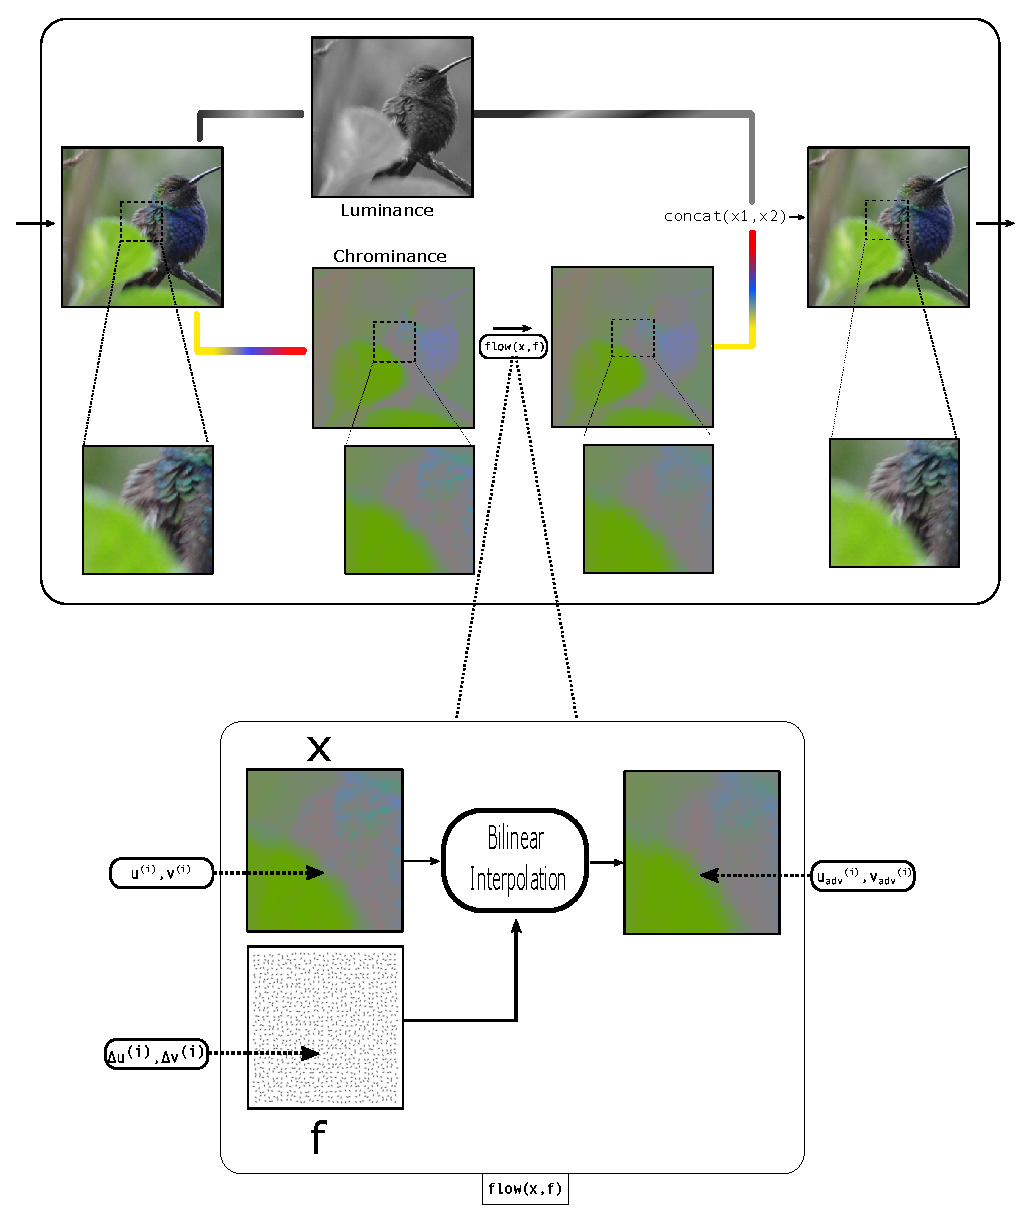
\includegraphics[width=0.8\linewidth]{illustration/drawing.eps}
    \caption[Visual illustration of the proposed adversarial example generation method.]{Visual illustration of the proposed adversarial example generation method. Luminance and chrominance channels are Y and \(C_{b}C_{r}\) when \(YC_{b}C_{r}\) colorspace and L and \(a^*b^*\) when CIELAB colorspace is used. Visual representation of flow field, subpixel restriction by \(\tanh\) and conversion of concatenated image back to RGB colorspace is omitted for brevity.}\label{fig:algorithm}
\end{figure*}

\RestyleAlgo{ruled}
\begin{algorithm}[t]
    \caption{Adversarial example generation by spatial transformation in chrominance channels in a perceptual colorspace. }\label{alg1}
    \KwIn{   \(x\)

    }
    \KwOut{   \(x_{adv}\)}
    \KwData{
        target\_class,
        model,
        \(\kappa\),
        colorspace,
        max\_iters,
        is\_restricted,
    }
    \(f \sim \mathcal{N}(0,\,\sigma^{2})\)\;
    \(i \gets 0\);

    \While{\(i < max\_iters\)}{
    \If{\(colorspace == YC_{b}C_{r}\)}{
    \(x_{color} \gets to\_ycbcr(x)\)\;
    }
    \If{\(colorspace == CIELAB\)}{
        \(x_{color} \gets to\_lab(x)\)\;
    }
    \(x_{luma}, x_{chroma} \gets splitchannels(x_{color})\)\;
    \If{is\_restricted}{\(f \gets \tanh(f)\)}
    \(x_{chroma} \gets apply\_flow(x_{chroma}, f)\)\;
    \(x_{adv} \gets concat(x_{luma}, x_{chroma})\)\;
    \(x_{adv} \gets to\_rgb(x_{adv})\)\;
    \(adv\_scores = model(x_{adv})\)\;
    \(loss \gets loss\_fn(adv\_scores, target\_class, \kappa)\)\;
    \eIf{\(loss \leq \kappa\)}
    {\Return{\(x_{adv}\)}\;}
    {

        \(backprop(loss)\)\;
        \(update(f)\)\;
        \(i \gets i + 1\)\;
    }
    }
\end{algorithm}

\subsection{Application of Flow Field}
Flow field is applied to the benign image following the methodology in~\cite{xiao2018spatially} also explained in Chapter~\ref{chp:2_literature}. For each pixel in adversarial image \(i_{adv}\), corresponding flow field vector value \(p_{i,j}\) is added to the pixel location. Then, the corresponding pixel at the added location is sampled. Since the added location is not an integer, bilinear interpolation is used to sample from the fractional pixel locations. Bilinear interpolation also makes the method end-to-end differentiable, thus optimizable by gradient based optimizers.
%\subsubsection{Restricting the flow field}

\subsection{Chrominance Restriction of Flow Field}
Since applying a flow field to all channels or luminance channels of an image of perceptual colorspace yields visual distortions shown in Figure~\ref{fig:flowtochannels}, the flow field is only applied to the chrominance channels where human vision is not very sensitive to the information loss~\cite{vorobyev2004ecology} to make the adversarially perturbed images indistinguishable from their benign counterparts. Since widely used RGB colorspace is not designed to be a perceptual colorspace, even small spatial perturbations to any RGB channel creates visually distinguishable changes. Hence, we first convert the benign image to a perceptual colorspace such as \(YC_{b}C_{r}\) where human vision is not sensitive to the spatial perturbations in, which is \(C_{b}\) and \(C_{r}\) in \(YC_{b}C_{r}\), and \(a^*\) and \(b^*\) in CIELAB colorspace. Then, we apply the flow field only to the channels Cb and Cr in \(YC_{b}C_{r}\), and A and B in CIELAB colorspace.

\subsection{Subpixel Restriction of Flow Field}
As mentioned in Chapter~\ref{chp:1_introduction}, chroma subsampling effectively causes the same chroma values to be used in the neighboring pixels by removing the local variation of chrominance. This method is widely used in visual lossy compression standards since the resolution loss in chrominance components of an image often does not cause any artifacts visible by a human observer. Accordingly, to exploit this fact, we can impose a restriction to the flow field to keep its values in the range \((-1, 1)\). We initialize a pre-flow field \(f_{pre}\) and calculate the applied flow field as \(f = \tanh(f_{pre})\). This differentiable reparameterization~\cite{mordvintsev2018differentiable} of flow field constraints the flow field magnitude to be smaller than 1 without inhibiting end-to-end differentiability so that chrominance value of each pixel of the adversarial image \(x_{adv}\) is only affected by the value of the pixel of the same location in \(x\) and its neighboring pixels. %With this modification, chroma subsampling becomes a very effective defense method to the subpixel restricted variant our attack without making any visually perceptible changes, as discussed in Section~\refeq{section:discussion}.


% In many multimedia compression standards such as JPEG and MPEG, chroma components are usually subsampled to compress information without making visually perceptible changes.


